\documentclass[12pt]{article}

\usepackage[brazil]{babel}   
\usepackage[utf8]{inputenc}  
%\usepackage[T1]{fontenc}
\usepackage{amsfonts,amsmath,amssymb,latexsym} 
\usepackage{float}
\usepackage{graphicx}
\graphicspath{ {images/} }

\def\cQ{\mathcal{Q}}
\def\ve{\varepsilon}

\def\emptyset{\varnothing}



\title{Lista 03 de ATC}
\date{}
%\date{2º Período de 2023}
\author{Turma do 3º ano}

\begin{document} 

\maketitle

\begin{description}

\item[Operadores de Expressões Regulares]:
\begin{itemize}
\item A união de duas linguagens $L$ e $M$ denotada por $L\cup M$ 
é o conjunto de strings que estão em $L$ ou em $M$
\item A concatenação de duas linguagens $L$ e $M$ denotada por $LM$
é o conjunto de strings que podem ser formados concatenando-se qualquer string de $L$ 
com qualquer string de $M$, 
nesta ordem
\item A potência $L^i$, para $i=0,1,2,3, \dots$; é a concatenação de $L$ com $L^{i-1}$, se $i>0$;
e $L^0 = \{\ve\}$ para $i=0$.
\item O fechamento de uma linguagem $L$, denotado por $L^*$ é a união
\[\bigcup_{i=0}^\infty L^i\]
\end{itemize}

\item[Definição de uma Expressão Regular (ER)]:

\begin{itemize}
\item $\emptyset$ é uma ER; $L(\emptyset) = \emptyset$.
\item $\ve$ é uma ER; $L(\ve) = \{\ve\}$.
\item \textbf{a} é uma ER, $a\in \Sigma$; $L($\textbf{a}$) = \{a\}$.
\item Se $E$ e $F$ são ER, então $E+F$ é ER; $L(E+F) = L(E)\cup L(F)$.
\item Se $E$ e $F$ são ER, então $EF$ é ER; $L(EF) = L(E)L(F)$.
\item Se $E$ é ER, então $E^*$ é ER; $L(E^*) = L(E)^*$.
\item Se $E$ é ER, então $(E)$ é ER; $L((E)) = L(E)$.
\end{itemize}

\break

\item[ER para AFN$\ve$]:
\begin{itemize}
\item $\emptyset$
\begin{figure}[H]
    \centering
    \includegraphics[width=0.4\textwidth]{ERtoAFNeEmpty}
    \caption{$\emptyset$}
    \label{fig:ERtoAFNeEmpty}
\end{figure}

\item $\ve$
\begin{figure}[H]
    \centering
    \includegraphics[width=0.4\textwidth]{ERtoAFNeVarep}
    \caption{$\ve$}
    \label{fig:ERtoAFNeVarep}
\end{figure}

\item $a$
\begin{figure}[H]
    \centering
    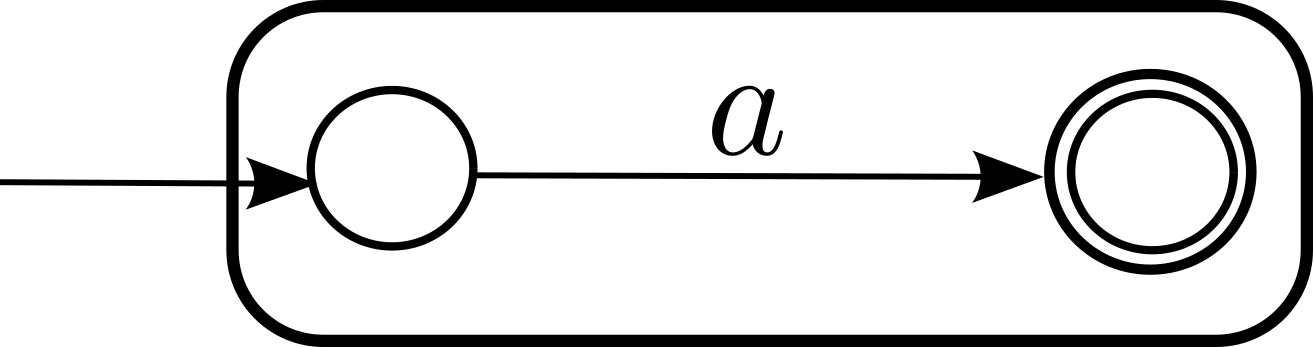
\includegraphics[width=0.4\textwidth]{ERtoAFNea}
    \caption{$a\in \Sigma$}
    \label{fig:ERtoAFNea}
\end{figure}

\item $E+F$
\begin{figure}[H]
    \centering
    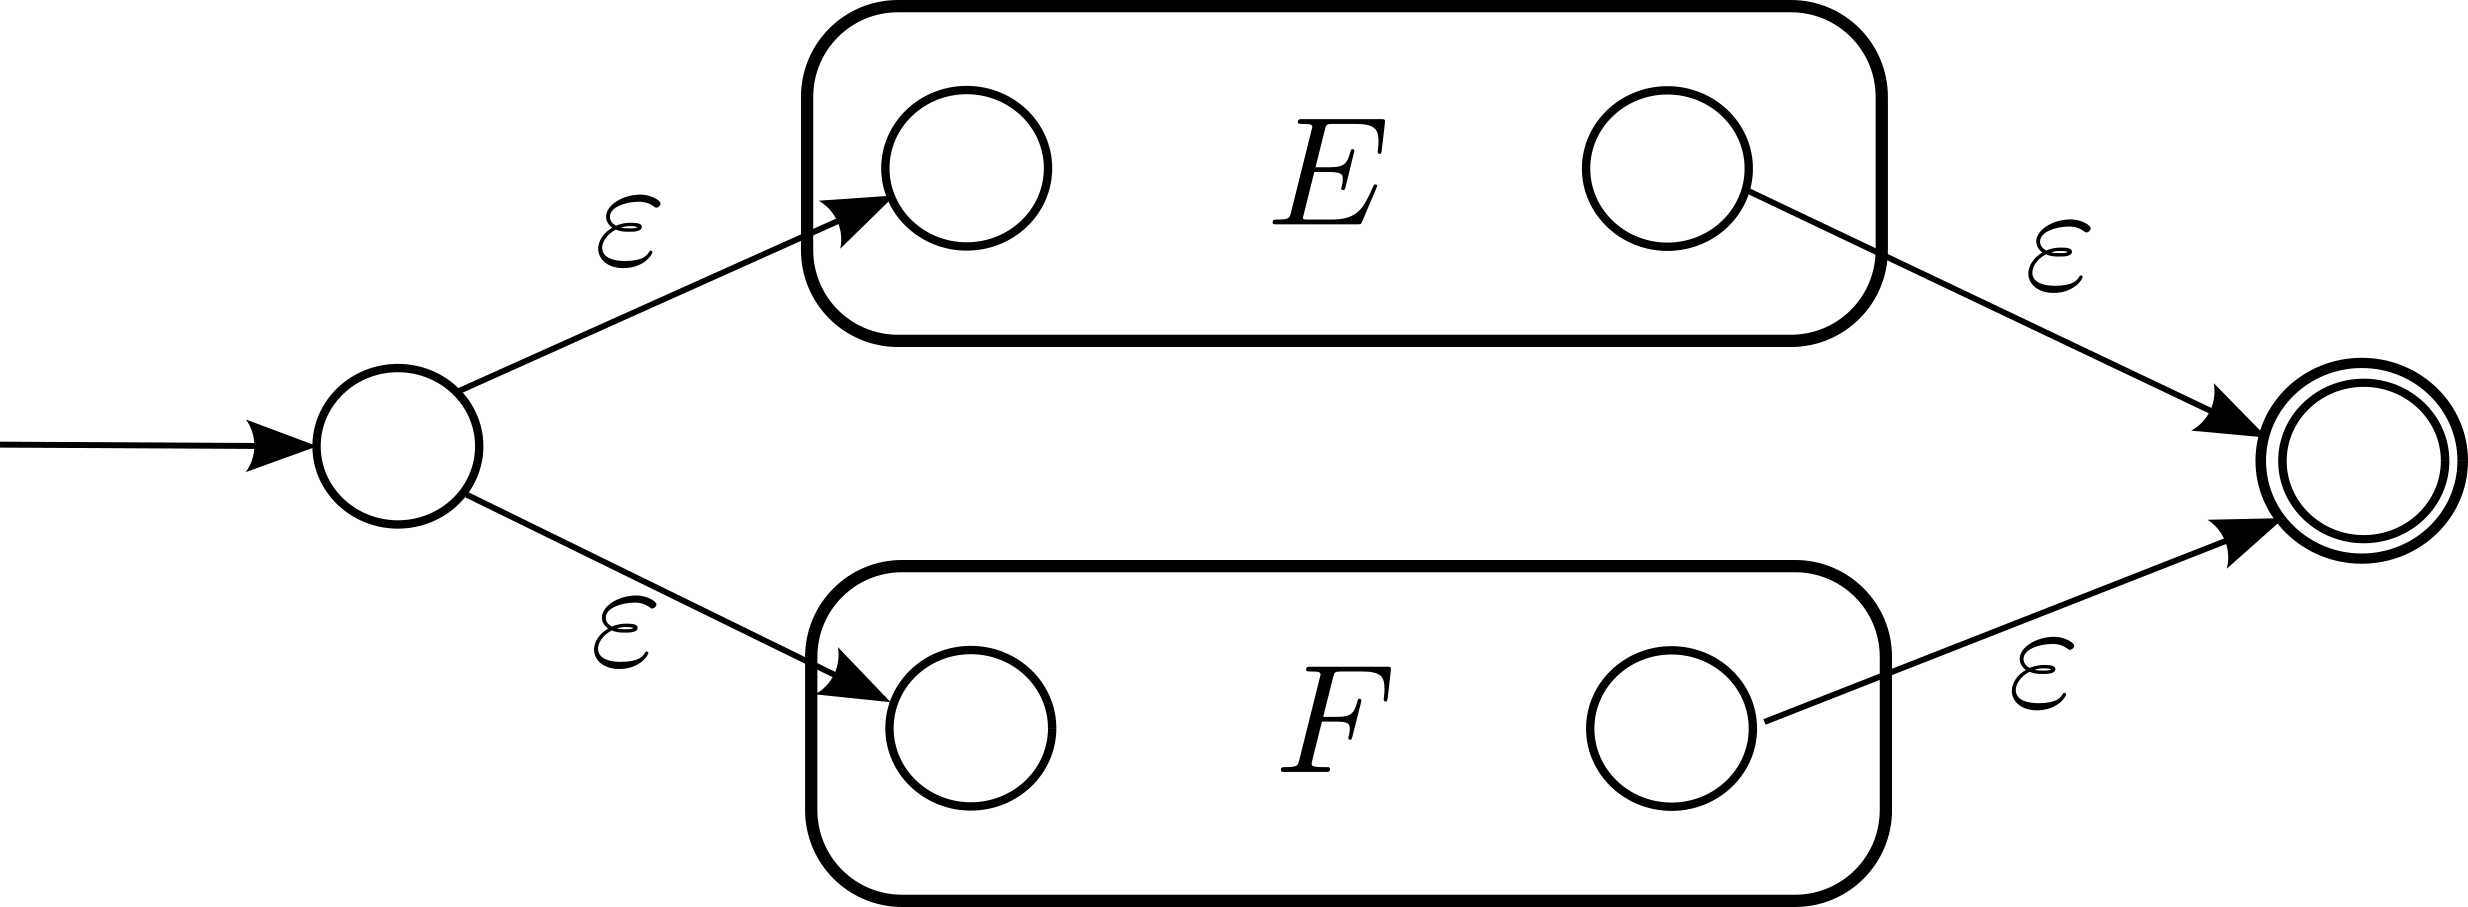
\includegraphics[width=0.6\textwidth]{ERtoAFNeE+F}
    \caption{$E+F$}
    \label{fig:ERtoAFNeE+F}
\end{figure}


\break

\item $EF$
\begin{figure}[H]
    \centering
    \includegraphics[width=0.6\textwidth]{ERtoAFNeEF}
    \caption{$EF$}
    \label{fig:ERtoAFNeEF}
\end{figure}

\item $E^*$
\begin{figure}[H]
    \centering
    \includegraphics[width=0.7\textwidth]{ERtoAFNeEKle}
    \caption{$E^*$}
    \label{fig:ERtoAFNeEKle}
\end{figure}


\end{itemize}


\end{description}

\vspace{3em}



\begin{enumerate}



\item Descreva em palavras as linguagens geradas pelas seguintes expressões regulares:

\begin{enumerate}

\item $(00^*1)^*0^*$

\item $(0^*1^*)^*000(0+1)^*$

\item $(0+10)^*$

\item $(a+b+c)^*(a+b+c)$

\item $(aa+b)^*$

\item $(b+ab)^*(\ve+a)$

\item $c^*(a+b)(a+b+c)^*$

\item $((b+c)^*+a(b+c)^*a)^*$

%\item $(aa+bb+(aa+bb)(ab+ba)(aa+bb))^*$

\end{enumerate}





\break





\item Desenvolva ER que gerem as seguintes linguagens sobre o alfabeto $\Sigma = \{0,1,+,-\}$

\begin{enumerate}

\item Expressões em uma linguagem tipo C, onde os operadores são $+$ ou $-$ e os números são binários.

\item Número inteiros em uma linguagem tipo C, composto por qualquer sequência não vazia de dígitos, precedido ou não por um sinal.

\end{enumerate}




\item Desenvolva ER que gerem as seguintes linguagens sobre o alfabeto $\Sigma = \{a,b,c\}$:

$\{w~|~w $ tem pelo menos um $a$ e um $b$ $\}$


\item Desenvolva ER que gerem as seguintes linguagens sobre o alfabeto $\Sigma = \{a,b\}$:

\begin{enumerate}

\item $\{w~|~w$ o terceiro símbolo a partir da extremidade direita é $a$ $\}$

%\item $\{w~|~w $ tem, no máximo, um par de $a$ como substring$\}$

%\item $\{w~|~w $ tem, no máximo, um par de $a$ como substring e um par de $b$ como substring$\}$

%\item $\{w~|~w $ não possui $aba$ como substring$\}$

%\item $\{w~|~$ qualquer par de $a$ antecede qualquer par de $b$ $\}$

\end{enumerate}




\item Quais das seguintes ER são equivalentes

\begin{enumerate}

\item $(a+b)^*a^*$
\item $(a+b)^*$
\item $((a+b)a)^*$


\end{enumerate}



\item Converta as expressões a seguir em AFD (Autômato Finito Determinístico, você pode primeiro transformar para AFD$\ve$ depois para AFD):

\begin{enumerate}

\item $01^*$

\item $(0+1)01$

\item $00(0+1)^*$

\end{enumerate}


%\item Quais linguagens tem o fechamento finito? (Forneça $L$ tal que $L^*$ é um conjunto finito)(são duas linguagens)


%\item Seja $E$ uma ER que gera a linguagem $L(E)$, que linguagens são geradas pelas seguintes expressões?

%\begin{enumerate}

%\item $\emptyset + E$

%\item $\ve E$

%\item $\emptyset E$

%\end{enumerate}





\end{enumerate}

\end{document}

